% % % % \input{DataFlow}

\subsection{Data Flow Viewpoint}

\begin{itemize}
\item Related stakeholders: KLM, Initiator
\item Related Concerns: Data Integrity, Performance, Scalability
\item Related design decisions: How is the data split up into multiple databases?; How do we handle large data-sets?; Recalculate or Combine rating?; Incremental or Time-interval update?; Flight-Information
\end{itemize}

\newpage
\begin{landscape}
\begin{figure}
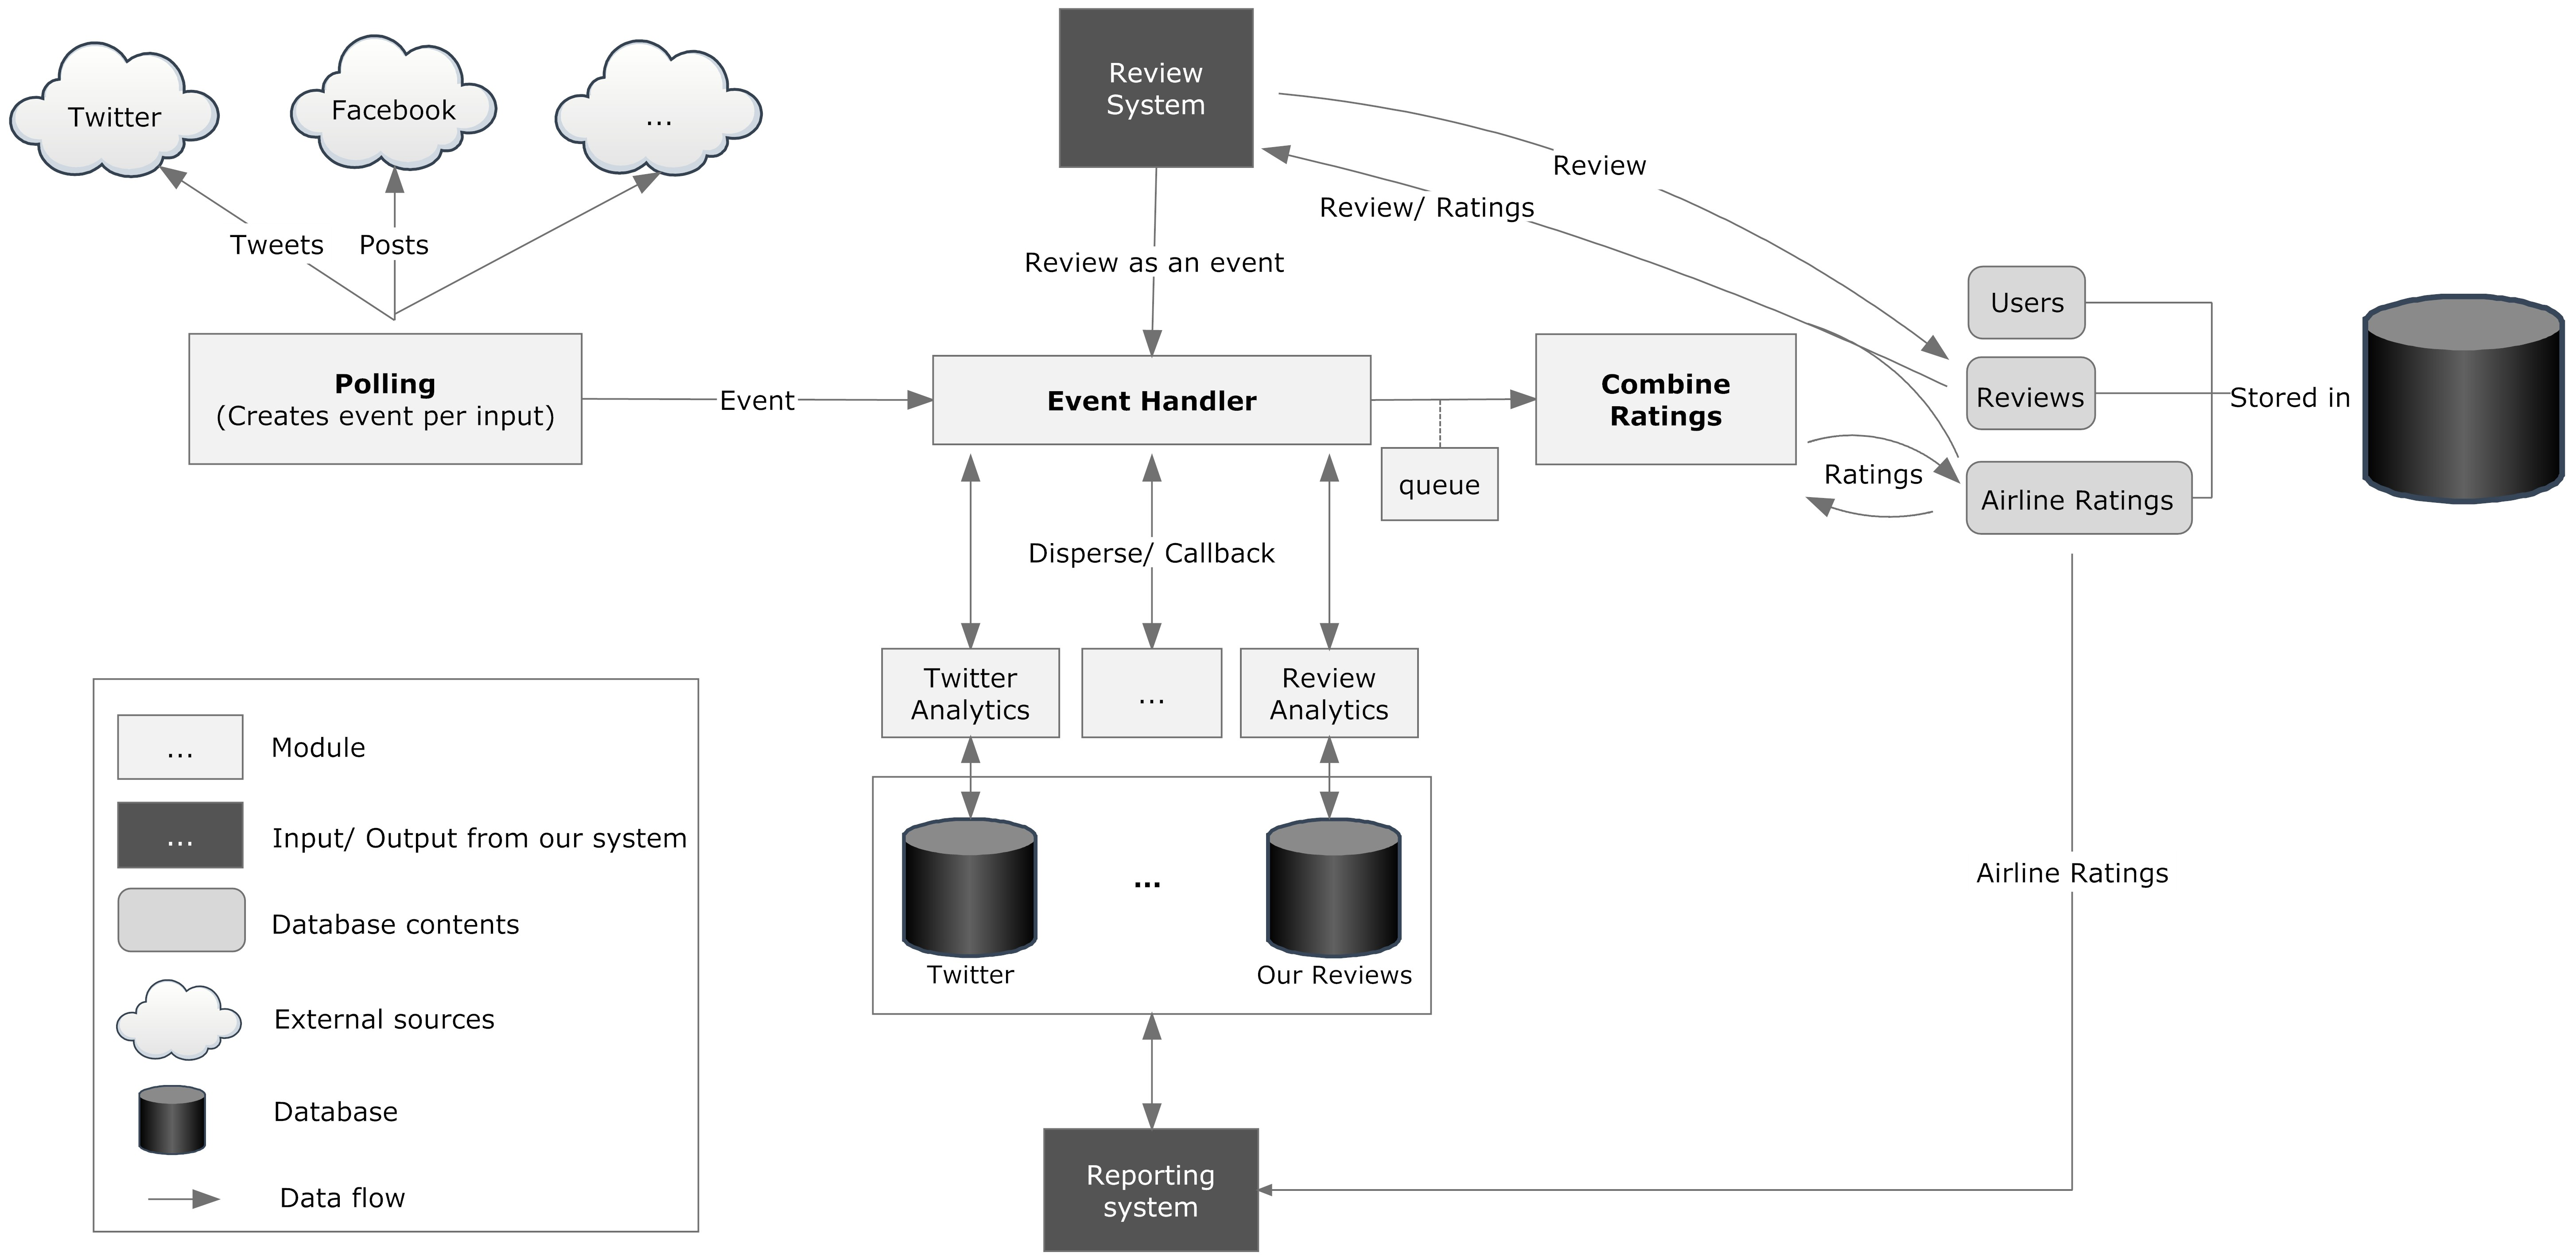
\includegraphics[width=600px]{DataFlowGraph}
\caption{Data Flow Viewpoint}
\label{fig:Data Flow}
\end{figure}
\end{landscape}

This Data Flow viewpoint \ref{fig:Data Flow} illustrates the flow of data within the back-end of the system. In this picture the review and reporting system are shown as black boxes to illustrate that their functionality is of no importance in this picture.
In the related design decisions it was argued that combining the rating with incremental updates was best for performance and scalability. Note that in the flow only the back-end of the system is given, because of the importance of handling the large data sets. Each of the modules and arrows in the viewpoint are explained here after.

\subsubsection{Polling}
The polling module is responsible for obtaining reviews from external data sources. It polls every external source on a given time-frame which is different for each external source. The reviews are not formatted and there original data format from the external source is kept. The rationale behind this decision is that all the reviews from external sources are significantly different of each other. Parsing them into a general format would lead to data loss or lots of undefined fields. The decision is further elaborated in the appendix at \ref{dd:save-raw}. The unformatted reviews are then passed on to the event handler as events. An event is defined as a single unformatted review either from external or internal sources.

\subsubsection{Event handler}
The event handler receives the events from both the polling module (external sources) and the review system (internal source). The responsibility of the event handler is to send these events to the analytics module specific to that data source. The event handler allows for parallel processing of reviews and greatly increased the performance and scalability compared to a more traditional pipeline model. This decision is further elaborated on in the appendix at \ref{dd:large-data}.

\subsubsection{Analytics}
Each data source has its own analytics module, because the data must be treated differently from external sources as they are of different format. The separate analytics modules have the added benefit of allowing for meta-analysis specific to a given data source. An example could be the amount of followers on twitter.

The analytics module analyses the unformatted review and produces a rating on a given scale for a certain or multiple categories (Overall, food, timeliness etc.). The unformatted review together with the analysed ratings are then stored in the analytics database of the data source. This is a requirement by the Initiator and KLM. The decision is further discussed in the appendix \ref{dd:data-format}. The ratings are also send of the combine ratings module in order to update the rating of the airline that is related to the review.

\subsubsection{Combine Ratings}
The combine ratings module is responsible for combining the ratings from the individual reviews into a final rating for an airline. The module receives the ratings from the analytics module and obtains the old rating from the main database. These two are combined in order to form a new rating. The process of iteratively combining ratings instead of recalculating is made for performance reasons as it is much cheaper and efficient to not recalculate the ratings that are already in the final rating of the airline. This decision is discussed in the appendix at \ref{dd:recalc-comb}. The ratings are based on an airline and a specific category (overall, timeliness, food etc.).

\subsubsection{Modules}
The functionality of each of the modules is discussed in the functional view. Hence in this section only the data flow regarding each of the modules is discussed:

\begin{enumerate}
\item \emph{R \& R module} A new review is inserted as event into the event handler which can pass it off to the specific analytics module. The decision was made to save the internal reviews twice: once in the main database and once when the they are analysed in the Analytics database. This allows the users to see the reviews without accessing the analytics database, but increases overhead as the same data is almost saved twice.
\item \emph{Reporting module} The reporting module retrieves information from the analytics database which contain all the analysed data together with the raw reviews. It must also be able to access the main database for the latest final ratings.
\item \emph{Authentication module} The user data for logging purposes is saved in the main database. The data contains sensitive information and is therefore encrypted.
\item \emph{Billing module} In order to make a profit airlines need to pay for their functionality. Therefore the billing module is able to read the current enlisted airlines and write to the database if the airlines have paid or not.
\item \emph{Messaging module} The messages are saved separately in the main database. Because they can contain user sensitive information (e.g. Flight numbers, names) the whole messages are saved in an encrypted form.
\end{enumerate}


\subsection{Data Flow Viewpoint}

\begin{itemize}
\item Related stakeholders: KLM, Initiator
\item Related Concerns: Data Integrity, Performance, Scalability
\item Related design decisions: How is the data split up into multiple databases?; How do we handle large data-sets?; Recalculate or Combine rating?; Incremental or Time-interval update?; Flight-Information
\end{itemize}

\newpage
\begin{landscape}
\begin{figure}
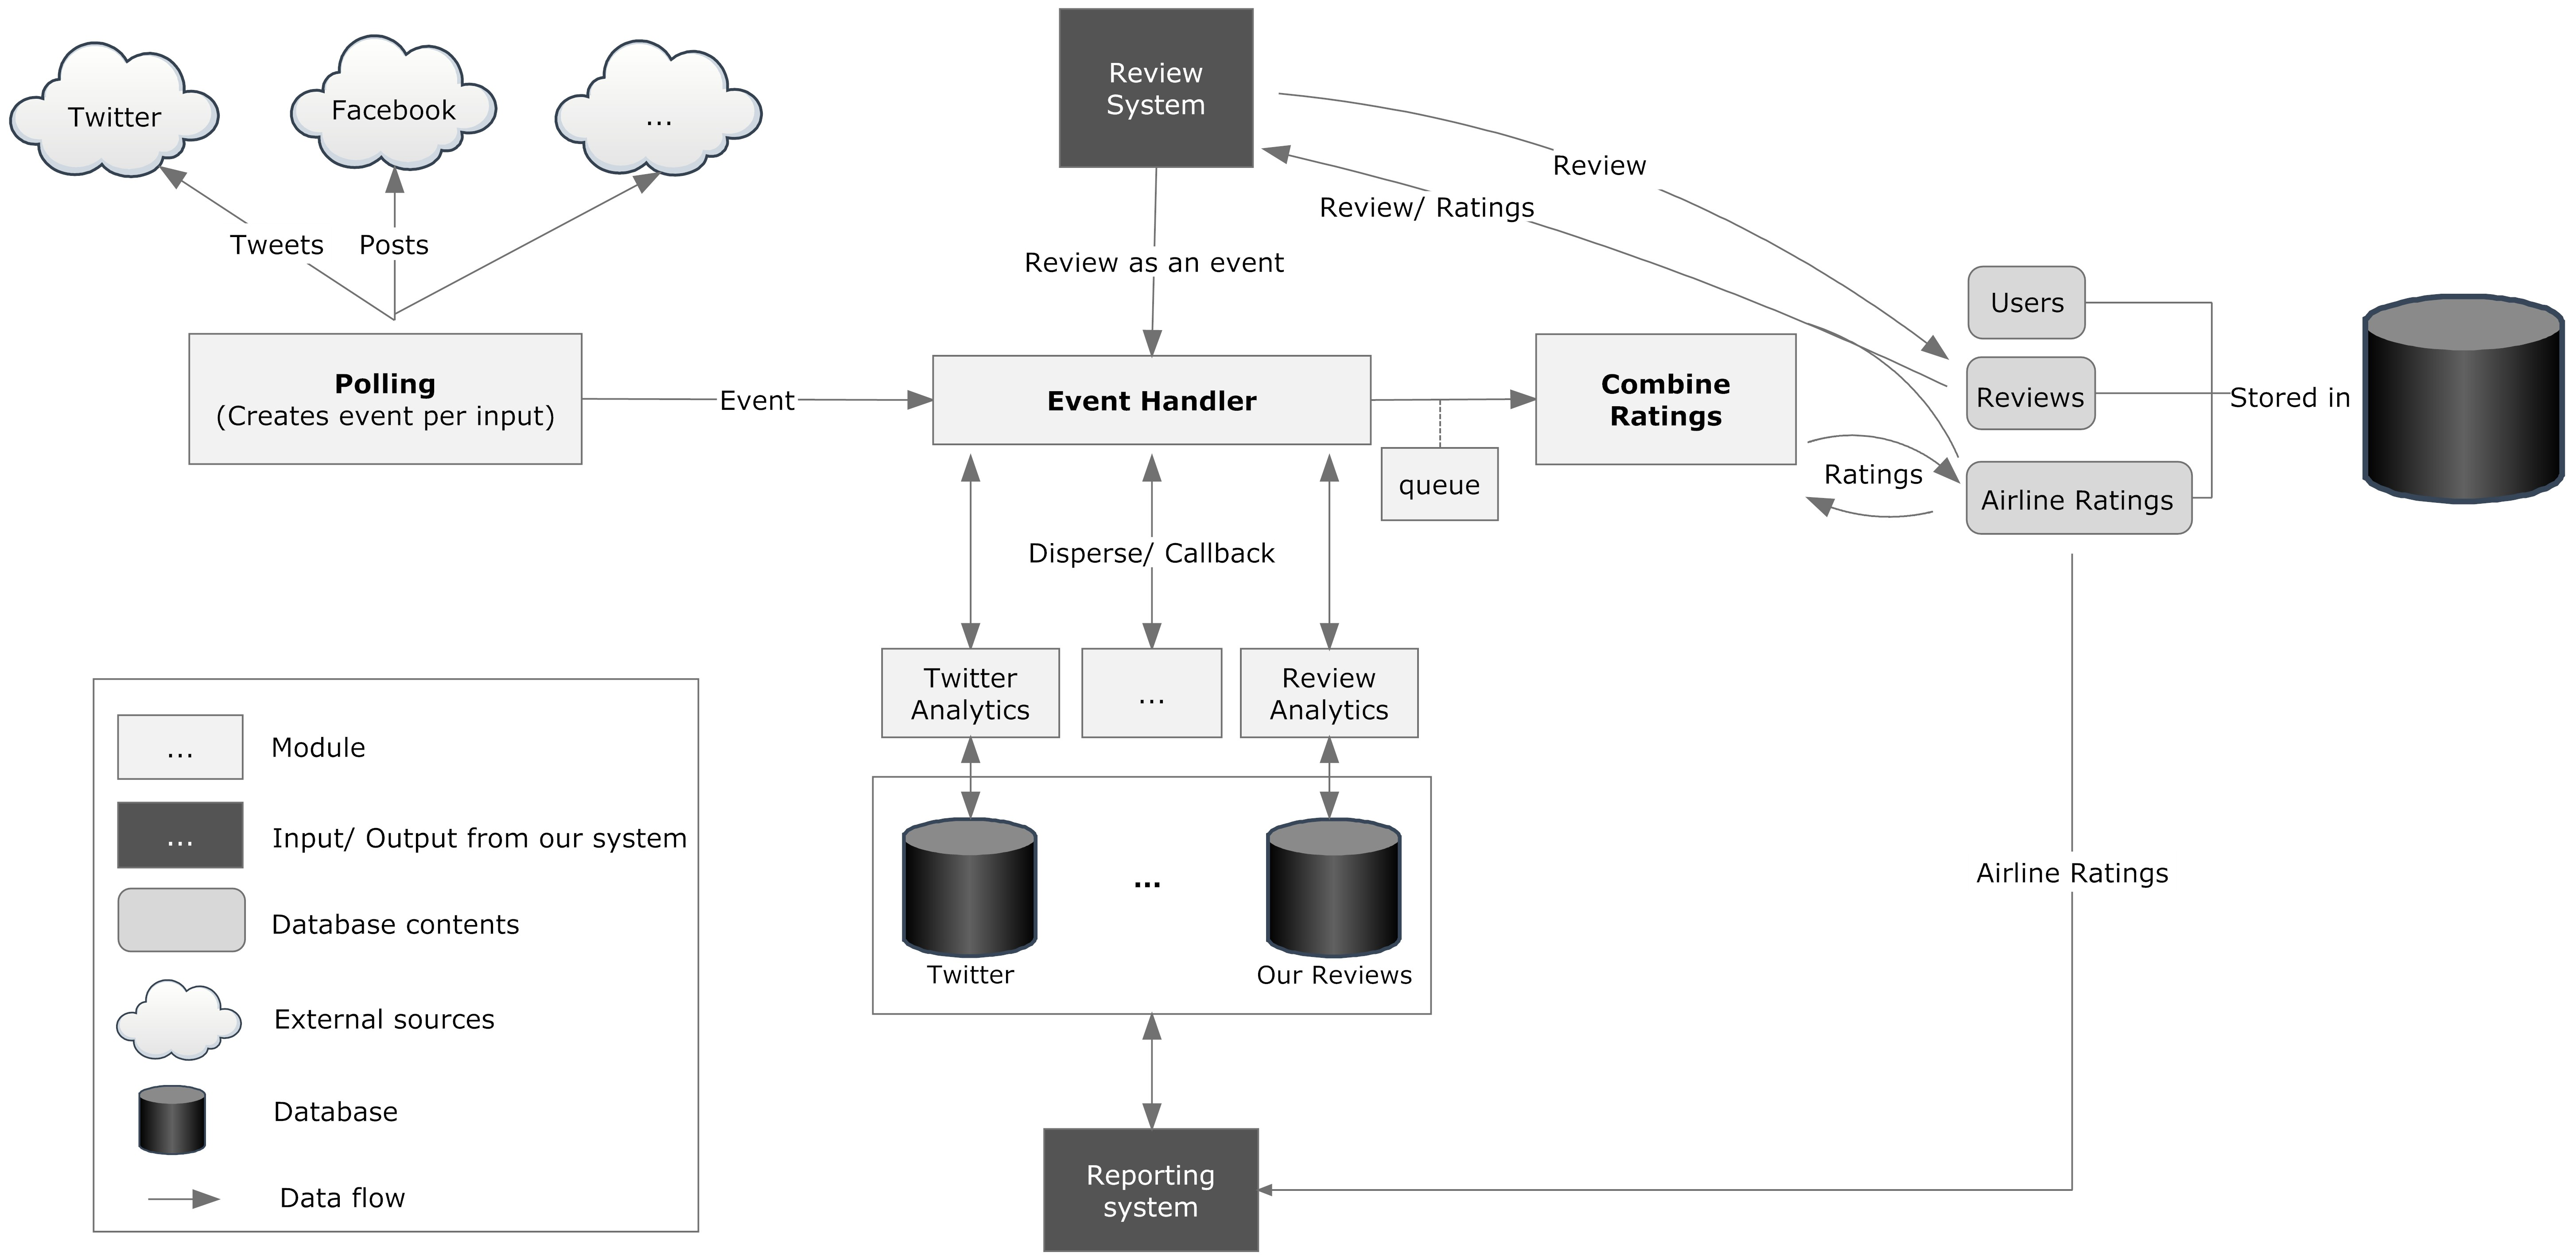
\includegraphics[width=600px]{DataFlowGraph}
\caption{Data Flow Viewpoint}
\label{fig:Data Flow}
\end{figure}
\end{landscape}

This Data Flow viewpoint \ref{fig:Data Flow} illustrates the flow of data within the back-end of the system. In this picture the review and reporting system are shown as black boxes to illustrate that their functionality is of no importance in this picture.
In the related design decisions it was argued that combining the rating with incremental updates was best for performance and scalability. Note that in the flow only the back-end of the system is given, because of the importance of handling the large data sets. Each of the modules and arrows in the viewpoint are explained here after.

\subsubsection{Polling}
The polling module is responsible for obtaining reviews from external data sources. It polls every external source on a given time-frame which is different for each external source. The reviews are not formatted and there original data format from the external source is kept. The rationale behind this decision is that all the reviews from external sources are significantly different of each other. Parsing them into a general format would lead to data loss or lots of undefined fields. The decision is further elaborated in the appendix at \ref{dd:save-raw}. The unformatted reviews are then passed on to the event handler as events. An event is defined as a single unformatted review either from external or internal sources.

\subsubsection{Event handler}
The event handler receives the events from both the polling module (external sources) and the review system (internal source). The responsibility of the event handler is to send these events to the analytics module specific to that data source. The event handler allows for parallel processing of reviews and greatly increased the performance and scalability compared to a more traditional pipeline model. This decision is further elaborated on in the appendix at \ref{dd:large-data}.

\subsubsection{Analytics}
Each data source has its own analytics module, because the data must be treated differently from external sources as they are of different format. The separate analytics modules have the added benefit of allowing for meta-analysis specific to a given data source. An example could be the amount of followers on twitter.

The analytics module analyses the unformatted review and produces a rating on a given scale for a certain or multiple categories (Overall, food, timeliness etc.). The unformatted review together with the analysed ratings are then stored in the analytics database of the data source. This is a requirement by the Initiator and KLM. The decision is further discussed in the appendix \ref{dd:data-format}. The ratings are also send of the combine ratings module in order to update the rating of the airline that is related to the review.

\subsubsection{Combine Ratings}
The combine ratings module is responsible for combining the ratings from the individual reviews into a final rating for an airline. The module receives the ratings from the analytics module and obtains the old rating from the main database. These two are combined in order to form a new rating. The process of iteratively combining ratings instead of recalculating is made for performance reasons as it is much cheaper and efficient to not recalculate the ratings that are already in the final rating of the airline. This decision is discussed in the appendix at \ref{dd:recalc-comb}. The ratings are based on an airline and a specific category (overall, timeliness, food etc.).

\subsubsection{Modules}
The functionality of each of the modules is discussed in the functional view. Hence in this section only the data flow regarding each of the modules is discussed:

\begin{enumerate}
\item \emph{R \& R module} A new review is inserted as event into the event handler which can pass it off to the specific analytics module. The decision was made to save the internal reviews twice: once in the main database and once when the they are analysed in the Analytics database. This allows the users to see the reviews without accessing the analytics database, but increases overhead as the same data is almost saved twice.
\item \emph{Reporting module} The reporting module retrieves information from the analytics database which contain all the analysed data together with the raw reviews. It must also be able to access the main database for the latest final ratings.
\item \emph{Authentication module} The user data for logging purposes is saved in the main database. The data contains sensitive information and is therefore encrypted.
\item \emph{Billing module} In order to make a profit airlines need to pay for their functionality. Therefore the billing module is able to read the current enlisted airlines and write to the database if the airlines have paid or not.
\item \emph{Messaging module} The messages are saved separately in the main database. Because they can contain user sensitive information (e.g. Flight numbers, names) the whole messages are saved in an encrypted form.
\end{enumerate}


\subsection{Data Flow Viewpoint}

\begin{itemize}
\item Related stakeholders: KLM, Initiator
\item Related Concerns: Data Integrity, Performance, Scalability
\item Related design decisions: How is the data split up into multiple databases?; How do we handle large data-sets?; Recalculate or Combine rating?; Incremental or Time-interval update?; Flight-Information
\end{itemize}

\newpage
\begin{landscape}
\begin{figure}
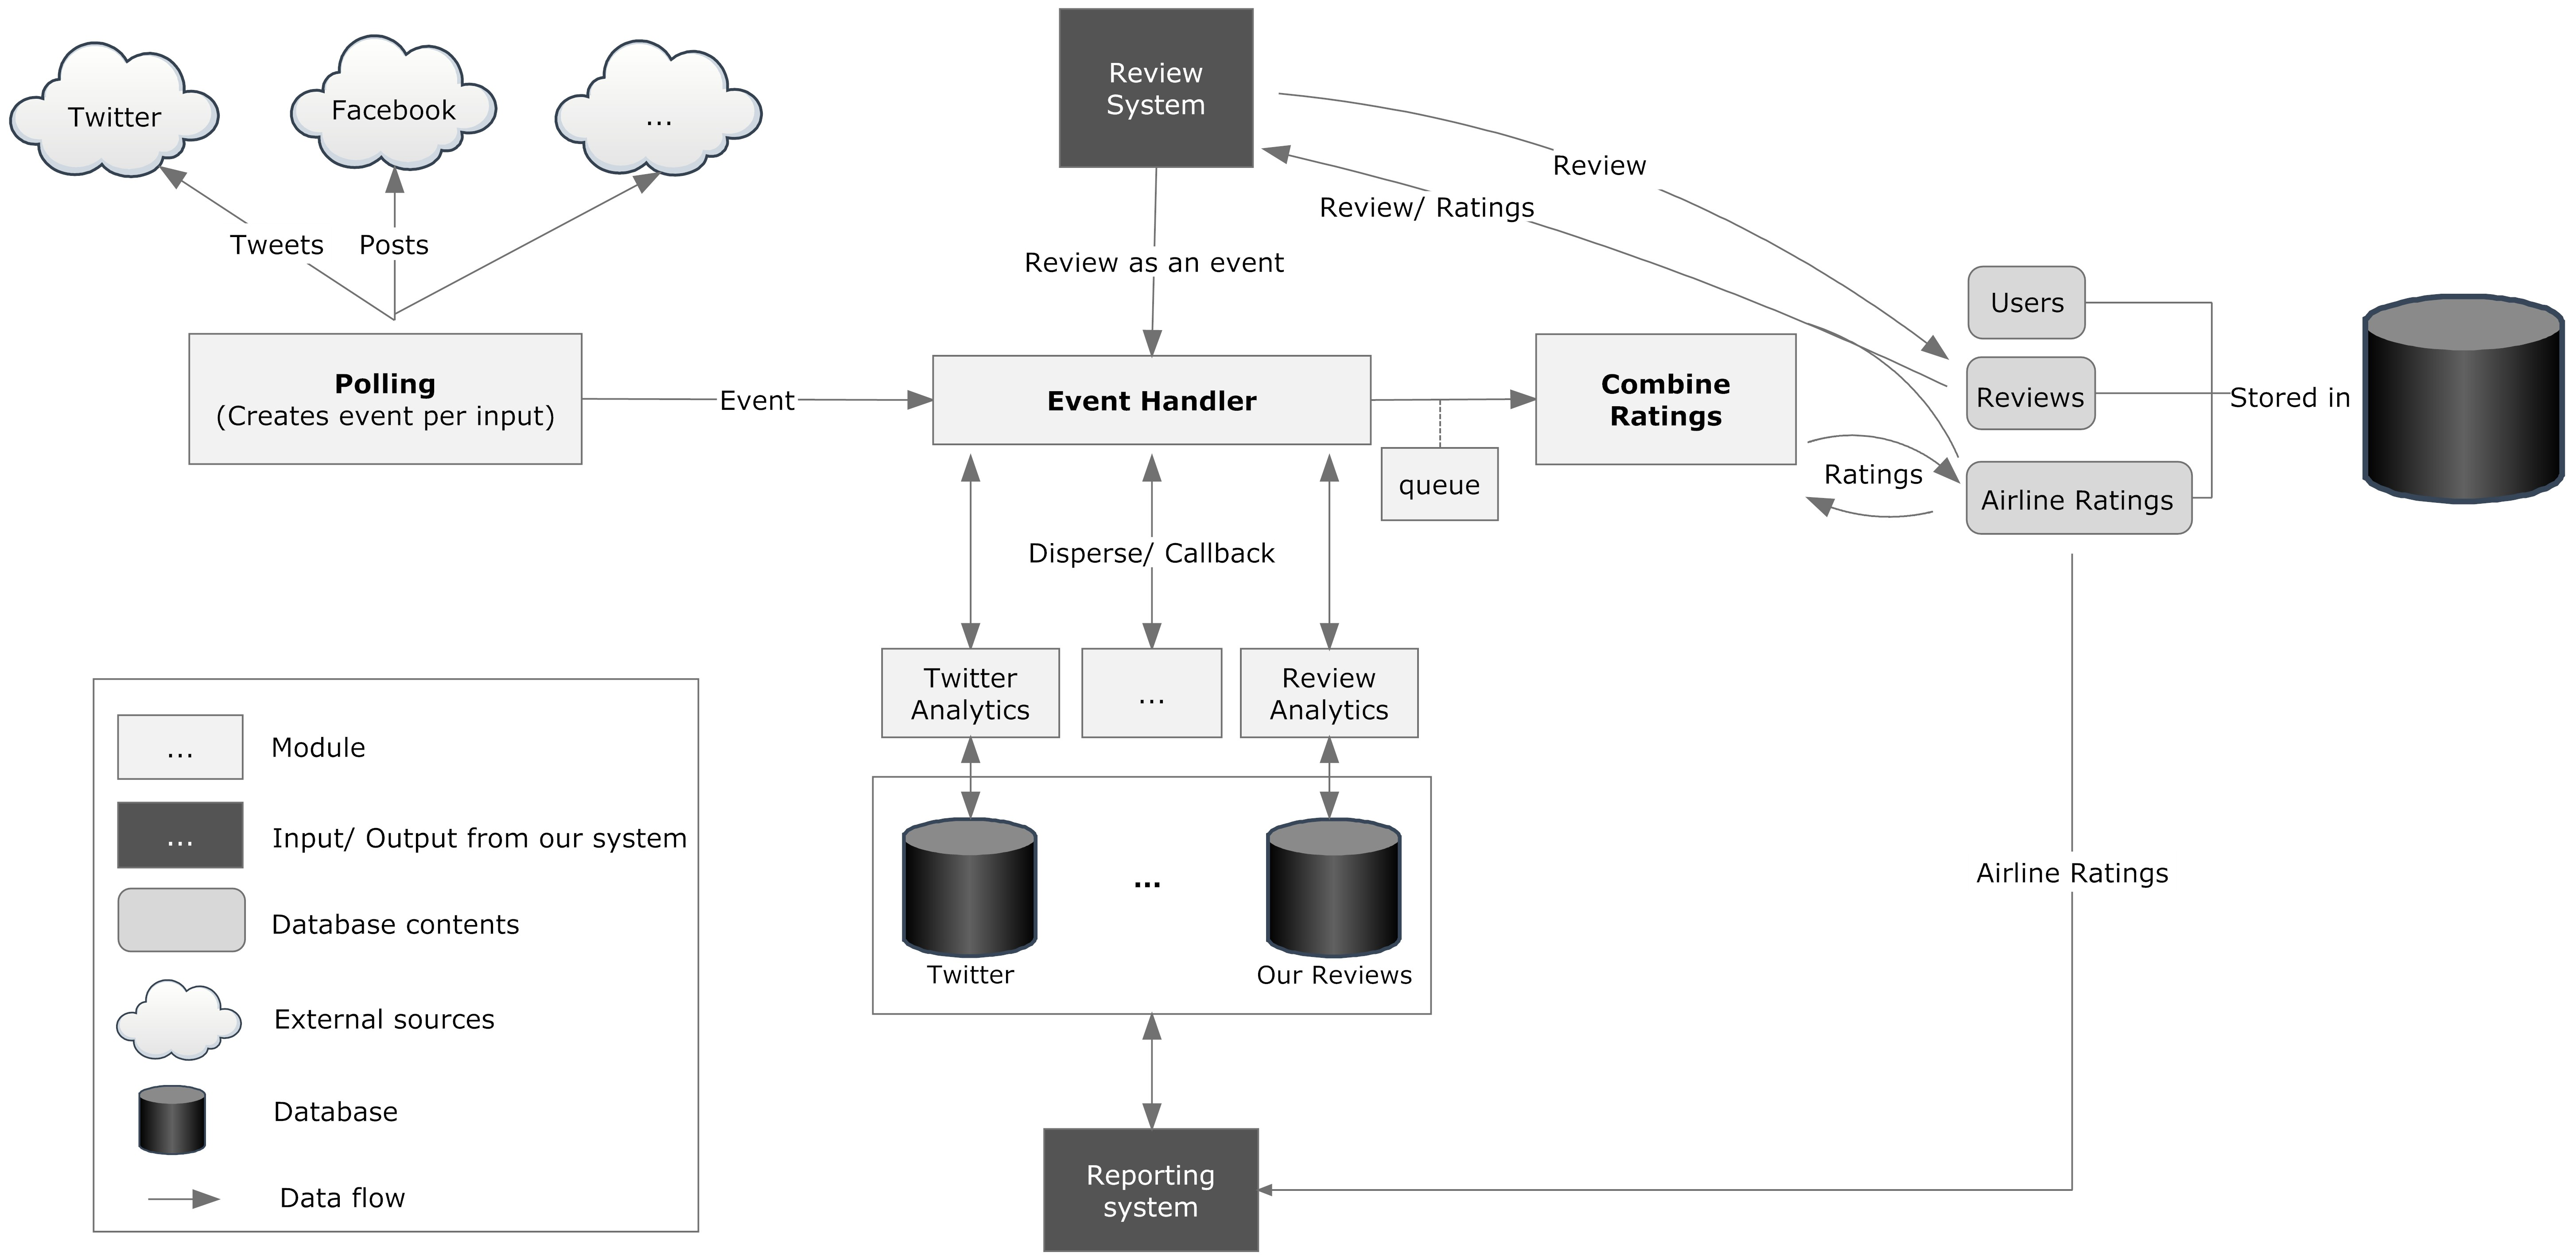
\includegraphics[width=600px]{DataFlowGraph}
\caption{Data Flow Viewpoint}
\label{fig:Data Flow}
\end{figure}
\end{landscape}

This Data Flow viewpoint \ref{fig:Data Flow} illustrates the flow of data within the back-end of the system. In this picture the review and reporting system are shown as black boxes to illustrate that their functionality is of no importance in this picture.
In the related design decisions it was argued that combining the rating with incremental updates was best for performance and scalability. Note that in the flow only the back-end of the system is given, because of the importance of handling the large data sets. Each of the modules and arrows in the viewpoint are explained here after.

\subsubsection{Polling}
The polling module is responsible for obtaining reviews from external data sources. It polls every external source on a given time-frame which is different for each external source. The reviews are not formatted and there original data format from the external source is kept. The rationale behind this decision is that all the reviews from external sources are significantly different of each other. Parsing them into a general format would lead to data loss or lots of undefined fields. The decision is further elaborated in the appendix at \ref{dd:save-raw}. The unformatted reviews are then passed on to the event handler as events. An event is defined as a single unformatted review either from external or internal sources.

\subsubsection{Event handler}
The event handler receives the events from both the polling module (external sources) and the review system (internal source). The responsibility of the event handler is to send these events to the analytics module specific to that data source. The event handler allows for parallel processing of reviews and greatly increased the performance and scalability compared to a more traditional pipeline model. This decision is further elaborated on in the appendix at \ref{dd:large-data}.

\subsubsection{Analytics}
Each data source has its own analytics module, because the data must be treated differently from external sources as they are of different format. The separate analytics modules have the added benefit of allowing for meta-analysis specific to a given data source. An example could be the amount of followers on twitter.

The analytics module analyses the unformatted review and produces a rating on a given scale for a certain or multiple categories (Overall, food, timeliness etc.). The unformatted review together with the analysed ratings are then stored in the analytics database of the data source. This is a requirement by the Initiator and KLM. The decision is further discussed in the appendix \ref{dd:data-format}. The ratings are also send of the combine ratings module in order to update the rating of the airline that is related to the review.

\subsubsection{Combine Ratings}
The combine ratings module is responsible for combining the ratings from the individual reviews into a final rating for an airline. The module receives the ratings from the analytics module and obtains the old rating from the main database. These two are combined in order to form a new rating. The process of iteratively combining ratings instead of recalculating is made for performance reasons as it is much cheaper and efficient to not recalculate the ratings that are already in the final rating of the airline. This decision is discussed in the appendix at \ref{dd:recalc-comb}. The ratings are based on an airline and a specific category (overall, timeliness, food etc.).

\subsubsection{Modules}
The functionality of each of the modules is discussed in the functional view. Hence in this section only the data flow regarding each of the modules is discussed:

\begin{enumerate}
\item \emph{R \& R module} A new review is inserted as event into the event handler which can pass it off to the specific analytics module. The decision was made to save the internal reviews twice: once in the main database and once when the they are analysed in the Analytics database. This allows the users to see the reviews without accessing the analytics database, but increases overhead as the same data is almost saved twice.
\item \emph{Reporting module} The reporting module retrieves information from the analytics database which contain all the analysed data together with the raw reviews. It must also be able to access the main database for the latest final ratings.
\item \emph{Authentication module} The user data for logging purposes is saved in the main database. The data contains sensitive information and is therefore encrypted.
\item \emph{Billing module} In order to make a profit airlines need to pay for their functionality. Therefore the billing module is able to read the current enlisted airlines and write to the database if the airlines have paid or not.
\item \emph{Messaging module} The messages are saved separately in the main database. Because they can contain user sensitive information (e.g. Flight numbers, names) the whole messages are saved in an encrypted form.
\end{enumerate}


\subsection{Concurrency Viewpoint}

\begin{itemize}
\item Related stakeholders: KLM, Initiator
\item Related Concerns: Availability, Performance, GreenIT
\item Related design decisions: Redudancy; Concurrency
\end{itemize}

\newpage
\begin{landscape}
\begin{figure}
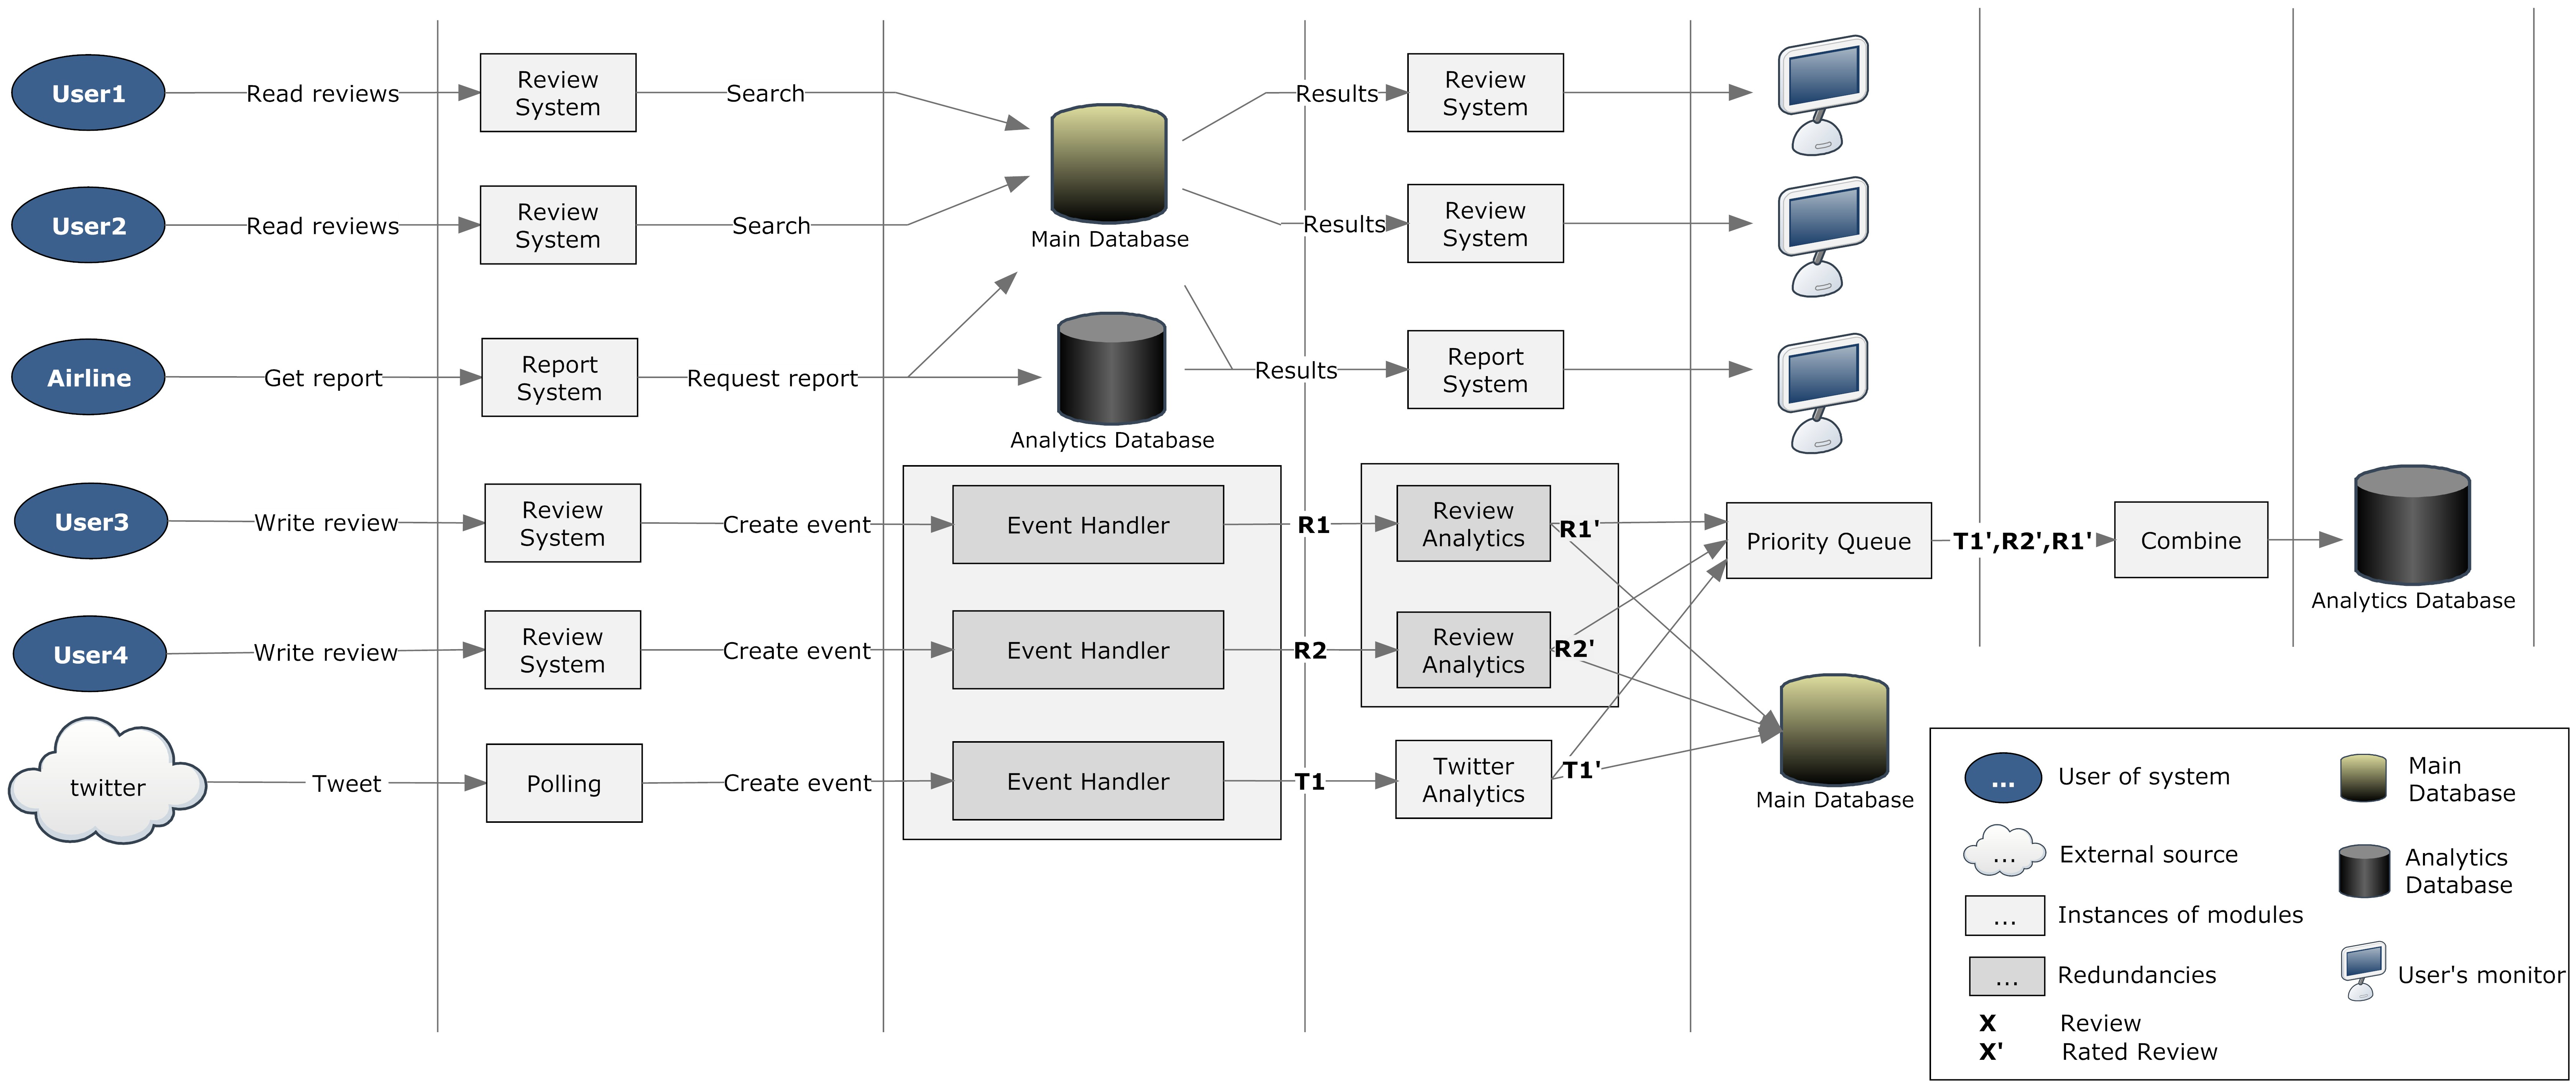
\includegraphics[width=600px]{ConcurrencyViewpoint.jpg}
\caption{Concurrency Viewpoint}
\label{fig:concurrency}
\end{figure}
\end{landscape}

The concurrency viewpoint (see fig.~\ref{fig:concurrency}) illustrates how the system behaves when different users perform different operations on it.the flow of data within the back-end of the system. In this figure the registered users or guests that search or read reviews are represented by the Users Reading element and the registered users that write a  review are represented as Users Writing. This separation is necessary because these operations are handled differently by the system since the writing operation changes the state of the database while the reading operation does not. The airlines are represented only by one entity because there is no need to separate the search or the statistics results since they are both reading operations and do not cause any change on the database's state. Finally, to represent the external sources we do not need to separate them since they are handled the same way by the system.

In the related design decisions it is discussed that redundancy will increase availability by eliminating single points of failure. Although it may decrease performance, it makes FlyWithUs a more robust system. 

\subsubsection{Instances of Modules}

A module's instances are separate processes that perform the same operations. For example, different instances of R\&R module respond to the users' requests, these instances can be different processes run on web servers. Additionally, instances of the modules review analytics and an external source analytics (eg. Facebook, Twitter, trip Advisor etc.) can run concurrently as different threads since the process of each post is dealt independently.

\subsubsection{Redundancies}

This viewpoint also puts forth single points of failure such as the event handler, the queue and the combine module. If any of these modules fails the system will have to revert to a previous state losing some the data collected. To avoid that, the system can have redundant modules that perform the same functionality and are synchronized, if any of them fails the others can continue from the point of failure without losing any data. Although it will increase the cost and will have negative impact on green IT, the stakeholders insisted on not losing any data and make the system as available as possible.
